%ten point, letter paper, single column
\documentclass[letterpaper,10pt, onecolumn, draftclsnofoot]{IEEEtran}

\usepackage{graphicx}                                        
\usepackage{amssymb}                                         
\usepackage{amsmath}                                         
\usepackage{amsthm}                                          

\usepackage{alltt}                                           
\usepackage{float}
\usepackage{color}
\usepackage{fancyvrb}
\usepackage{url}

\usepackage{balance}
\usepackage[TABBOTCAP, tight]{subfigure}
\usepackage{enumitem}
\usepackage{pstricks, pst-node}
\usepackage{listings}
\usepackage{tabularx}

\usepackage{geometry}
%0.75 in margin on each side, total of 1.5 in
\geometry{textheight=8.5in, textwidth=6in}
\usepackage{pgfgantt}

%random comment

\newcommand{\cred}[1]{{\color{red}#1}}
\newcommand{\cblue}[1]{{\color{blue}#1}}

\newcommand{\toc}{\tableofcontents}

%\usepackage{hyperref}

\def\name{Thomas Albertine}
\title{The Many Faces of Microbial Communities \\\large Senior Design\\Spring Term Final Report\\}
\author{\name, Michael Phelps}


%% The following metadata will show up in the PDF properties
% \hypersetup{
%   colorlinks = false,
%   urlcolor = black,
%   pdfauthor = {\name},
%   pdfkeywords = {capstone visualization microbiology microbio senior design},
%   pdftitle = {Senior Design Project, Visualizing Microbial Communities},
%   pdfsubject = {Senior Design Microbiology Visualizations},
%   pdfpagemode = UseNone
% }

\lstset{language=python,
                basicstyle=\ttfamily,
                keywordstyle=\color{blue}\ttfamily,
                stringstyle=\color{red}\ttfamily,
                commentstyle=\color{green}\ttfamily,
                morecomment=[l][\color{magenta}]{\#},
				breaklines=true,
				showstringspaces=false
}

\parindent = 0.0 in
\parskip = 0.1 in

%Single space
\linespread{1.0}

\usepackage{fancyvrb}
\usepackage{color}
\usepackage[latin1]{inputenc}


\makeatletter
\def\PY@reset{\let\PY@it=\relax \let\PY@bf=\relax%
    \let\PY@ul=\relax \let\PY@tc=\relax%
    \let\PY@bc=\relax \let\PY@ff=\relax}
\def\PY@tok#1{\csname PY@tok@#1\endcsname}
\def\PY@toks#1+{\ifx\relax#1\empty\else%
    \PY@tok{#1}\expandafter\PY@toks\fi}
\def\PY@do#1{\PY@bc{\PY@tc{\PY@ul{%
    \PY@it{\PY@bf{\PY@ff{#1}}}}}}}
\def\PY#1#2{\PY@reset\PY@toks#1+\relax+\PY@do{#2}}

\expandafter\def\csname PY@tok@gd\endcsname{\def\PY@tc##1{\textcolor[rgb]{0.63,0.00,0.00}{##1}}}
\expandafter\def\csname PY@tok@gu\endcsname{\let\PY@bf=\textbf\def\PY@tc##1{\textcolor[rgb]{0.50,0.00,0.50}{##1}}}
\expandafter\def\csname PY@tok@gt\endcsname{\def\PY@tc##1{\textcolor[rgb]{0.00,0.25,0.82}{##1}}}
\expandafter\def\csname PY@tok@gs\endcsname{\let\PY@bf=\textbf}
\expandafter\def\csname PY@tok@gr\endcsname{\def\PY@tc##1{\textcolor[rgb]{1.00,0.00,0.00}{##1}}}
\expandafter\def\csname PY@tok@cm\endcsname{\let\PY@it=\textit\def\PY@tc##1{\textcolor[rgb]{0.25,0.50,0.50}{##1}}}
\expandafter\def\csname PY@tok@vg\endcsname{\def\PY@tc##1{\textcolor[rgb]{0.10,0.09,0.49}{##1}}}
\expandafter\def\csname PY@tok@m\endcsname{\def\PY@tc##1{\textcolor[rgb]{0.40,0.40,0.40}{##1}}}
\expandafter\def\csname PY@tok@mh\endcsname{\def\PY@tc##1{\textcolor[rgb]{0.40,0.40,0.40}{##1}}}
\expandafter\def\csname PY@tok@go\endcsname{\def\PY@tc##1{\textcolor[rgb]{0.50,0.50,0.50}{##1}}}
\expandafter\def\csname PY@tok@ge\endcsname{\let\PY@it=\textit}
\expandafter\def\csname PY@tok@vc\endcsname{\def\PY@tc##1{\textcolor[rgb]{0.10,0.09,0.49}{##1}}}
\expandafter\def\csname PY@tok@il\endcsname{\def\PY@tc##1{\textcolor[rgb]{0.40,0.40,0.40}{##1}}}
\expandafter\def\csname PY@tok@cs\endcsname{\let\PY@it=\textit\def\PY@tc##1{\textcolor[rgb]{0.25,0.50,0.50}{##1}}}
\expandafter\def\csname PY@tok@cp\endcsname{\def\PY@tc##1{\textcolor[rgb]{0.74,0.48,0.00}{##1}}}
\expandafter\def\csname PY@tok@gi\endcsname{\def\PY@tc##1{\textcolor[rgb]{0.00,0.63,0.00}{##1}}}
\expandafter\def\csname PY@tok@gh\endcsname{\let\PY@bf=\textbf\def\PY@tc##1{\textcolor[rgb]{0.00,0.00,0.50}{##1}}}
\expandafter\def\csname PY@tok@ni\endcsname{\let\PY@bf=\textbf\def\PY@tc##1{\textcolor[rgb]{0.60,0.60,0.60}{##1}}}
\expandafter\def\csname PY@tok@nl\endcsname{\def\PY@tc##1{\textcolor[rgb]{0.63,0.63,0.00}{##1}}}
\expandafter\def\csname PY@tok@nn\endcsname{\let\PY@bf=\textbf\def\PY@tc##1{\textcolor[rgb]{0.00,0.00,1.00}{##1}}}
\expandafter\def\csname PY@tok@no\endcsname{\def\PY@tc##1{\textcolor[rgb]{0.53,0.00,0.00}{##1}}}
\expandafter\def\csname PY@tok@na\endcsname{\def\PY@tc##1{\textcolor[rgb]{0.49,0.56,0.16}{##1}}}
\expandafter\def\csname PY@tok@nb\endcsname{\def\PY@tc##1{\textcolor[rgb]{0.00,0.50,0.00}{##1}}}
\expandafter\def\csname PY@tok@nc\endcsname{\let\PY@bf=\textbf\def\PY@tc##1{\textcolor[rgb]{0.00,0.00,1.00}{##1}}}
\expandafter\def\csname PY@tok@nd\endcsname{\def\PY@tc##1{\textcolor[rgb]{0.67,0.13,1.00}{##1}}}
\expandafter\def\csname PY@tok@ne\endcsname{\let\PY@bf=\textbf\def\PY@tc##1{\textcolor[rgb]{0.82,0.25,0.23}{##1}}}
\expandafter\def\csname PY@tok@nf\endcsname{\def\PY@tc##1{\textcolor[rgb]{0.00,0.00,1.00}{##1}}}
\expandafter\def\csname PY@tok@si\endcsname{\let\PY@bf=\textbf\def\PY@tc##1{\textcolor[rgb]{0.73,0.40,0.53}{##1}}}
\expandafter\def\csname PY@tok@s2\endcsname{\def\PY@tc##1{\textcolor[rgb]{0.73,0.13,0.13}{##1}}}
\expandafter\def\csname PY@tok@vi\endcsname{\def\PY@tc##1{\textcolor[rgb]{0.10,0.09,0.49}{##1}}}
\expandafter\def\csname PY@tok@nt\endcsname{\let\PY@bf=\textbf\def\PY@tc##1{\textcolor[rgb]{0.00,0.50,0.00}{##1}}}
\expandafter\def\csname PY@tok@nv\endcsname{\def\PY@tc##1{\textcolor[rgb]{0.10,0.09,0.49}{##1}}}
\expandafter\def\csname PY@tok@s1\endcsname{\def\PY@tc##1{\textcolor[rgb]{0.73,0.13,0.13}{##1}}}
\expandafter\def\csname PY@tok@sh\endcsname{\def\PY@tc##1{\textcolor[rgb]{0.73,0.13,0.13}{##1}}}
\expandafter\def\csname PY@tok@sc\endcsname{\def\PY@tc##1{\textcolor[rgb]{0.73,0.13,0.13}{##1}}}
\expandafter\def\csname PY@tok@sx\endcsname{\def\PY@tc##1{\textcolor[rgb]{0.00,0.50,0.00}{##1}}}
\expandafter\def\csname PY@tok@bp\endcsname{\def\PY@tc##1{\textcolor[rgb]{0.00,0.50,0.00}{##1}}}
\expandafter\def\csname PY@tok@c1\endcsname{\let\PY@it=\textit\def\PY@tc##1{\textcolor[rgb]{0.25,0.50,0.50}{##1}}}
\expandafter\def\csname PY@tok@kc\endcsname{\let\PY@bf=\textbf\def\PY@tc##1{\textcolor[rgb]{0.00,0.50,0.00}{##1}}}
\expandafter\def\csname PY@tok@c\endcsname{\let\PY@it=\textit\def\PY@tc##1{\textcolor[rgb]{0.25,0.50,0.50}{##1}}}
\expandafter\def\csname PY@tok@mf\endcsname{\def\PY@tc##1{\textcolor[rgb]{0.40,0.40,0.40}{##1}}}
\expandafter\def\csname PY@tok@err\endcsname{\def\PY@bc##1{\setlength{\fboxsep}{0pt}\fcolorbox[rgb]{1.00,0.00,0.00}{1,1,1}{\strut ##1}}}
\expandafter\def\csname PY@tok@kd\endcsname{\let\PY@bf=\textbf\def\PY@tc##1{\textcolor[rgb]{0.00,0.50,0.00}{##1}}}
\expandafter\def\csname PY@tok@ss\endcsname{\def\PY@tc##1{\textcolor[rgb]{0.10,0.09,0.49}{##1}}}
\expandafter\def\csname PY@tok@sr\endcsname{\def\PY@tc##1{\textcolor[rgb]{0.73,0.40,0.53}{##1}}}
\expandafter\def\csname PY@tok@mo\endcsname{\def\PY@tc##1{\textcolor[rgb]{0.40,0.40,0.40}{##1}}}
\expandafter\def\csname PY@tok@kn\endcsname{\let\PY@bf=\textbf\def\PY@tc##1{\textcolor[rgb]{0.00,0.50,0.00}{##1}}}
\expandafter\def\csname PY@tok@mi\endcsname{\def\PY@tc##1{\textcolor[rgb]{0.40,0.40,0.40}{##1}}}
\expandafter\def\csname PY@tok@gp\endcsname{\let\PY@bf=\textbf\def\PY@tc##1{\textcolor[rgb]{0.00,0.00,0.50}{##1}}}
\expandafter\def\csname PY@tok@o\endcsname{\def\PY@tc##1{\textcolor[rgb]{0.40,0.40,0.40}{##1}}}
\expandafter\def\csname PY@tok@kr\endcsname{\let\PY@bf=\textbf\def\PY@tc##1{\textcolor[rgb]{0.00,0.50,0.00}{##1}}}
\expandafter\def\csname PY@tok@s\endcsname{\def\PY@tc##1{\textcolor[rgb]{0.73,0.13,0.13}{##1}}}
\expandafter\def\csname PY@tok@kp\endcsname{\def\PY@tc##1{\textcolor[rgb]{0.00,0.50,0.00}{##1}}}
\expandafter\def\csname PY@tok@w\endcsname{\def\PY@tc##1{\textcolor[rgb]{0.73,0.73,0.73}{##1}}}
\expandafter\def\csname PY@tok@kt\endcsname{\def\PY@tc##1{\textcolor[rgb]{0.69,0.00,0.25}{##1}}}
\expandafter\def\csname PY@tok@ow\endcsname{\let\PY@bf=\textbf\def\PY@tc##1{\textcolor[rgb]{0.67,0.13,1.00}{##1}}}
\expandafter\def\csname PY@tok@sb\endcsname{\def\PY@tc##1{\textcolor[rgb]{0.73,0.13,0.13}{##1}}}
\expandafter\def\csname PY@tok@k\endcsname{\let\PY@bf=\textbf\def\PY@tc##1{\textcolor[rgb]{0.00,0.50,0.00}{##1}}}
\expandafter\def\csname PY@tok@se\endcsname{\let\PY@bf=\textbf\def\PY@tc##1{\textcolor[rgb]{0.73,0.40,0.13}{##1}}}
\expandafter\def\csname PY@tok@sd\endcsname{\let\PY@it=\textit\def\PY@tc##1{\textcolor[rgb]{0.73,0.13,0.13}{##1}}}

\def\PYZbs{\char`\\}
\def\PYZus{\char`\_}
\def\PYZob{\char`\{}
\def\PYZcb{\char`\}}
\def\PYZca{\char`\^}
\def\PYZam{\char`\&}
\def\PYZlt{\char`\<}
\def\PYZgt{\char`\>}
\def\PYZsh{\char`\#}
\def\PYZpc{\char`\%}
\def\PYZdl{\char`\$}
\def\PYZti{\char`\~}
% for compatibility with earlier versions
\def\PYZat{@}
\def\PYZlb{[}
\def\PYZrb{]}
\makeatother


\begin{document}
\maketitle
\section{Abstract}

\clearpage

\tableofcontents

\section{Introduction}
Our client, Dr. Jenna Lang, a microbiology researcher from University of California Davis requested that we create a tool that she could use to visualize microbial population data as human faces. This tool could potentially help microbiology researchers (as well as those from other fields) find patterns that aren't obvious using existing visualization techniques. 

Currently, the standard visualizations are pie charts or heat maps. Unfortunately, Pie charts aren't effective when there are a large number of categories to represent because there are too many slices. Heat maps on the other hand, while still useful to see patterns, do not make proportions between organisms obvious the way pie charts do. Our tool takes advantage of the human brain's ability to recognize and interpret patterns in faces to visualize data, so users can find new patterns that they would normally miss.

Our team consisted of Thomas Albertine and Michael Phelps. We had no formal roles aside from ``developer'', although generally (but not exclusively) Thomas worked on the backend code, loading data files and generating models, while Michael worked on the frontend code, connecting the backend to a user interface (henceforth referred to as UI). Our client played a hands off role. We spoke with her early in the project to collect requirements and have contacted her to revisit requirements or to keep her aprised of how the project is going, but she generally gave usa lot of freedom regarding how to proceed.

\section{Original Requirements Document}
\begin{figure}[h]
	\begin{ganttchart}[vgrid={*1{black, dotted}}]{1}{21}
		\gantttitle{Initial Gantt Chart in Weeks}{21}\\
		\gantttitlelist{1,...,21}{1}\\
		
		%\ganttbar{Task Name}{start}{end}[name] \\
		%\ganttlink{name1}{name2 defaults to elem1 or the like}
		\ganttbar[name=exploremhuman]{Explore MakeHuman API}{1}{4} \\
		\ganttbar[name=fformats]{Explore File Formats}{1}{2} \\
		\ganttbar[name=lfile]{Load File}{3}{3}\\
		\ganttbar[name=mhumanwrapper]{MakeHuman Wrapper}{5}{8}\\
		\ganttbar[name=ldmodel]{Load and Draw Model}{11}{14}\\
		\ganttbar[name=ui]{Basic UI}{9}{10}\\
		\ganttbar[name=rpsmodel]{Rotate / Pan / Scale Model}{15}{16}\\
		\ganttbar[name=polish]{Polish UI}{17}{21}\\
		\ganttbar[name=expfsprt]{Expand File Type Support}{17}{21}\\
		
		\ganttlink{fformats}{lfile}
		\ganttlink{lfile}{mhumanwrapper}
		\ganttlink{exploremhuman}{mhumanwrapper}
		\ganttlink{mhumanwrapper}{ldmodel}
		\ganttlink{ui}{ldmodel}
		\ganttlink{ui}{polish}
		\ganttlink{ldmodel}{rpsmodel}
		\ganttlink{rpsmodel}{polish}
	\end{ganttchart}
	\caption{This is the original Gantt chart for the project.}
\end{figure}

\subsection{Requirements Document}
The Many Faces of Microbial Communities Project

Team Name: ViewCrobe Software

Members: Thomas Albertine, Michael Phelps

\subsubsection{Introduction}

\paragraph{Purpose}
The theory behind the project is that, since there is a specific portion of the human brain dedicated to processing faces, visualizing microbial data as faces allows users to better compare the complex data. Therefore, the purpose of the project is to provide that functionality in a tool usable primarily by microbiologists, but secondarily by researchers in other disciplines.

\paragraph{Scope}
FaceView will be a user-friendly tool for providing visualizations of microbial population data by representing data as 3d models of humans. Given a supported data file, FaceView will allow the user to select a subset of samples from the file from which to generate models based on a subset of the various populations in the file. After these models are generated, these models will be draw to the screen for comparison by users.

In order to enhance user-friendliness, sample subsets will be relatively small for ease of comparison, while population subsets will be significantly larger to allow for more comprehensive comparisons.

\paragraph{Definitions, Acronyms, and Abbreviations}
\begin{itemize}
	\item Model--In the context of this project, ``model'' refers to a 3 dimensional representation of a human based on a subset of the input data. Since a given model is generated from a sample, in some contexts, the two terms may be interchangeable. 
	\item Sample--In the context of an input file, a sample is a subset of the data representing one population. As an example, a sample may contain the number of colonies and which species they are associated with in a petri dish.
	\item Common Camera Angles--A set of configurations for the observer of a 3d scene that are used often. Such a set would include a front view, a profile view, and a three-quarter view at least.
	\item Visualization Profiles--Data files may include many samples and many organism populations. It may contain more populations than there are supported models or model parameters. Therefore it may become necessary to ignore some samples and some organism populations. Furthermore, the user may want to reassign the model parameter that corresponds to a given organism's population to better emphasize differences in that organism among the samples. However, manually modifying which model parameters correspond to which organisms and which samples should be ignored could be time-consuming to do each time. Therefore it may be expedient to create a profile of these settings, which could be saved and loaded later.
	\item Model Parameters--Values that can be passed in when generating a model in order to influence the outcome. For example, nose length might be a model parameter.
	\item Data Parameters--Values that are read from the data. These can be associated with model parameters to make the visualization reflect the data. For example, the population of E. Coli in a set of samples, which may be tied to the nose length in the finished model.
\end{itemize}

\subsubsection{Bibliography}

[1] ``Data Formats,'' [Online]. Available: \newline http://www.metagenassist.ca/METAGENassist/faces/Docs/Format.jsp. [Accessed 6 November 2015].

[2] ``The Magical Number Seven, Plus or Minus Two: Some Limits on our Capacity for Processing Information,'' Psychological Review, vol. 63, pp. 81-97, 1956. 

\subsubsection{Overall Description}
\paragraph{Product Perspective}

This project interacts with several other components. It reads and interprets supported data file formats. The minimal acceptable set of supported formats includes only the tab separated ``Classic QIIME OTU'' format [1], as it is sufficient for use. Expanding the set of supported file formats is a stretch goal. 

Additionally, we include a UI component to facilitate user interaction. This contains several components.

\begin{itemize}
	\item A screen in which the user will direct the application to a data file, a visualization profile which allows the user to configure which attributes are associated with which model features, and optionally a metadata file, containing groups of samples to aid in selection.
	\item A screen in which thumbnail images of the models will be drawn. This screen would also allow users to add and remove models from a group, and select models to be compared in more detail.
	\item A screen in which the selected models will be drawn. At this point, the user would be able to rotate, pan, and zoom around the models in order to better compare their features.
\end{itemize}

We recognize that certain additional features, while not absolutely necessary for a minimal functional product, would enhance usability, and therefore we add, as stretch goals, shortcuts to certain common camera angles, some way to save and load visualization profiles, and a way to export comparison images. Via our UI, a user from our target user group should be able to use our tool to produce their visualization in 5 minutes  or less with approximately 2 minutes or less of initial instruction. 

\begin{figure}[h]
	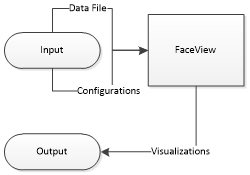
\includegraphics[width=0.4\textwidth]{functional.PNG}
	\caption{A Functional Diagram, demonstrating the interactions between the user and the application.}
	\label{fig:generated}
\end{figure}

\paragraph{Product Functions}
The project should support the following functions

\begin{itemize}
	\item The project should allow the user to select a subset of models to be drawn larger. Note that, in order to allow the user to easily identify similarities and differences in the drawn models, the number of models that can be drawn to the screen, and thus samples that can be represented at once, is limited to 6, since the maximum number of things a person can process at a given time is $7\pm2$ [2].
	\item The project should also support a thumbnail view to select models to view in more detail, and to add and remove models from groups.
	\item Similarly, the project should allow the user to select a subset of organisms to associate with certain module parameters, as those are limited by the number of model parameters that can be modified. 
	\begin{itemize}
		\item Furthermore the user should be able to choose which supported model parameters correspond with which organisms in the data file. This allows the user to allocate more obvious model features to the organisms he or she is most interested in.
	\end{itemize}
	\item The project should, using the data files and visualization profile, generate models and draw them to the screen.
	\item Once these models are drawn to the screen, the user should be able to rotate, pan, and zoom the views. The thumbnail view is exempt from this requirement, as that would make initial screening difficult.
\end{itemize}

\paragraph{User Characteristics}
Our intended users are researchers who are analyzing population data, specifically microbial population data. Such users are highly educated, but do not want to have to use unnecessarily complex or difficult tools.

\paragraph{Assumptions and Dependencies}
We assume that Windows will be installed on the machine running the project. We also assume a version of Python 3 is included.

\subsubsection{Specific Requirements}

\paragraph{Sample Subset}
The project should allow users to select a subset of at most 6 samples to compare in detail. This is to improve user-friendliness. Restricting the number of models shown may reduce distractions, allowing users to better compare certain samples. 

\paragraph{Grouping}
The project should allow users to organize samples into groups for easy profiling of features or comparing subsets of the data. Users should be able to add or remove samples from a given group.

\paragraph{Organism Subset}
The project should allow users to select a subset of organism appearing in the samples. This subset is limited by the number of model parameters which we can support, which should be at least 150. 

\paragraph{Model Parameter Assignment}
The project should allow users to specify certain model parameters to correspond to certain measurements in the data file, such as the population of a certain microbe corresponding to eye shape. This is to improve user-friendliness by allowing users to match parameters used in an existing result, or to allow certain features to be made more obvious.

\paragraph{Classic QIIME OTU Format Support}
Initially, the project should support the tab separated ``Classic'' QIIME OUT format for data files. It is human readable as it looks like a table when viewed in a text editor, which makes it a good choice for a proof of concept. Expanding file format support is a stretch goal. 

\paragraph{Transforming Data}
The project should transform the data from the data file into a format that can be used to generate the models. This allows us to produce a standard format for model generation, which allows us to expand supported file formats.

\paragraph{Producing a Model}
The project should produce a 3d human model based on the parameters from each selected sample. For each model generated in the batch, the same data parameter corresponds to the same model parameter. For example, if the population of a certain microbe in a certain sample corresponded to the straightness of the produced model's nose for that sample, then the population of the same microbe in a second sample would correspond to the straightness of its model's nose. This process should not take longer than 30 seconds.

\paragraph{Drawing Models}
The project should draw the produced models to the screen such that each of the models are viewable at the same time. This is to facilitate the user comparing models.

\paragraph{User Controls}
The project should allow users to rotate, pan, and zoom around the models in order to better compare them. All models should rotate, pan, and zoom.

\subsubsection{Additional ``Stretch'' Goals}

\paragraph{Provide a Web UI}
In addition to the local version, this would provide a web UI which would invoke the component that generates models on the server. These models would then be sent to the client browser to be presented to the user. This stretch goal would necessitate that the project be portable enough to run on a Linux server. 

\paragraph{Export Images for Later Comparison}
This feature would allow users to not only compare samples in the same file, but also to compare to files compared earlier. However, this would allow the user the opportunity to associate different data parameters with different model parameters between the two results, which could lead to misleading results.

\paragraph{Save and Load Visualization Profiles}
This feature would allow users to save and load visualization profiles, configurations of which samples and organisms from a given file are to be used when generating the model, and which organism corresponds to which feature.

\subsubsection{A -- An Explanation of Prerequisites Apparent in the Preliminary Gantt Chart}
\begin{itemize}
	\item Exploring File Formats -- This is time dedicated to choosing a data file type and understanding how to interpret one of those files. It has no dependencies.
	\item Explore MakeHuman API -- This is time dedicated to learning how to use the MakeHuman project to create Human Models programmatically. It has no dependencies
	\item Load File -- This task is to write code to load a data file, and translate it into a standard format. Its prerequisite is to understand a file format.
	\item MakeHuman Wrapper -- This task is to write a wrapper around the MakeHuman project so that we can send the parameters included in the standard parameter format into the project to generate a model. Its prerequisites are to explore the MakeHuman project and to generate the set of standard parameters.
	\item Basic UI -- This task is to create a basic UI through which the user will interact with the other components. Obviously, this will need to be connected to those components so one will be a prerequisite of the other. However, this one has no prerequisites because we need to be able to start somewhere.
	\item Load and Draw Model -- This task is to be able to load and draw a model generated by the MakeHuman project. It's prerequisite is a UI to draw it in.
	\item Rotate, Pan, Scale Model -- This task is to be able to apply the specified transformations to the model, allowing the user to better examine it. It's prerequisite is to be able to load and draw the models.
	\item Expand File Type Support -- This stretch goal is to support more file types. As it is a stretch goal, we would not work on it until we have satisfied the rest of the goals, therefore its prerequisite is to be finished with the rest of the project, represented in the Gantt chart as tasks that are otherwise at the end of a prerequisite chain.
	\item Polish UI -- This stretch goal is to make general cosmetic and user friendliness related improvements to the UI. As another stretch goal, its prerequisites are the same as the other's.
\end{itemize}

\section{Final Requirements Document}

\section{Design Document}

\section{Tech Review}

\section{Blog Posts}

\section{Poster}

\section{Project Documentation}

\section{Learning New Technologies}

\section{Personal Learning}
\subsection{Thomas Albertine}

\subsection{Michael Phelps}

\appendix[Essential Code Listings]

\appendix[Additional Content]

\end{document}
